\subsection{Enveloping Distribution Sampling (EDS)}
In EDS, free-energy differences between multiple end states are obtained by sampling a reference-state Hamiltonian, i.e. without the definition of specific alchemical paths \cite{Christ2007,Christ2008,Riniker2011}. 
Given $N$ end states, the potential energy function $V$ of the EDS reference state $R$ is defined as,
\begin{equation}
    V_R(\vec{r}; s, \vec{E}^R)= - \frac{1}{\beta s}\ln \left[ \sum^N_{i=1}{e^{-\beta s \left(V_i(\vec{r})- E_i^R\right) }} \right] ,
    \label{EQ: Reference EDS}
\end{equation}
where $\beta = (k_\mathrm{B} T)^{-1}$ with $k_\mathrm{B}$ being the Boltzmann constant and $T$ the absolute temperature.
The smoothing parameter $s$ and the energy offsets $\vec{E}^R$ were introduced to enable tuning of the reference state for optimal sampling of all end states \cite{Christ2007, Christ2008}.

%% $s$-parameter    
A smoothness parameter set to $s=1.0$ gives a reference potential-energy landscape that contains all the relevant minima of the end states. However, these might be separated by high barriers.
For $s < 1$, the energy barriers between different end states $V_i$ are smoothed in the reference potential $V_R$, increasing the transition rates between the different minima (Figure \ref{fig: EDS_potential_behavioura}) \cite{Christ2008}. 
However, if $s$ is chosen too small, $V_R$ consists of a global unphysical minimum, which does not correspond to any of the end states. 
In the limit of $s\rightarrow 0$, all end states contribute equally to the potential-energy function of the reference state \cite{Koenig2020}, which can lead to unphysical deformations. The situation with a too small $s$ has been termed ``undersampling'' \cite{Riniker2011}.



%%Eoff
The energy offsets $\vec{E}^R$ are used to ensure equal weighting of all end states $V_i$ in $V_R$ (Figure \ref{fig: EDS_potential_behaviourb}). 
Note that the optimal values of $s$ and $\vec{E}^R$ are not independent of each other (as can be seen in Eq. (\ref{EQ: Reference EDS})) \cite{Christ2008}.
%
Different schemes have been proposed to determine optimal reference-state parameters \cite{Riniker2011, Christ2009, Hansen2012}, however, these are only applicable to systems with two end states.

\begin{figure}[h]
    \begin{center}
    \begin{subfigure}{0.44\columnwidth}
        \centering
        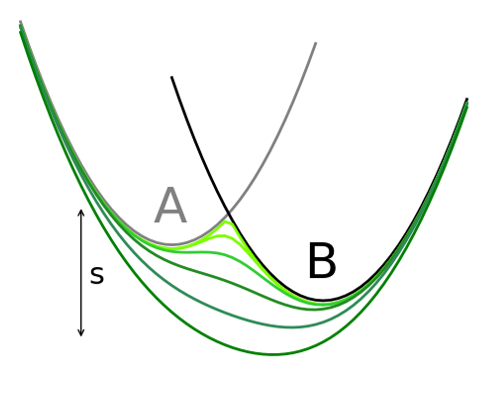
\includegraphics[width=\textwidth]{fig/intro/EDS_parmeters_s.png}
        \caption{Effect of $s$ on $V_R$}
        \label{fig: EDS_potential_behavioura}
    \end{subfigure}
    \begin{subfigure}{0.44\columnwidth}
        \centering
        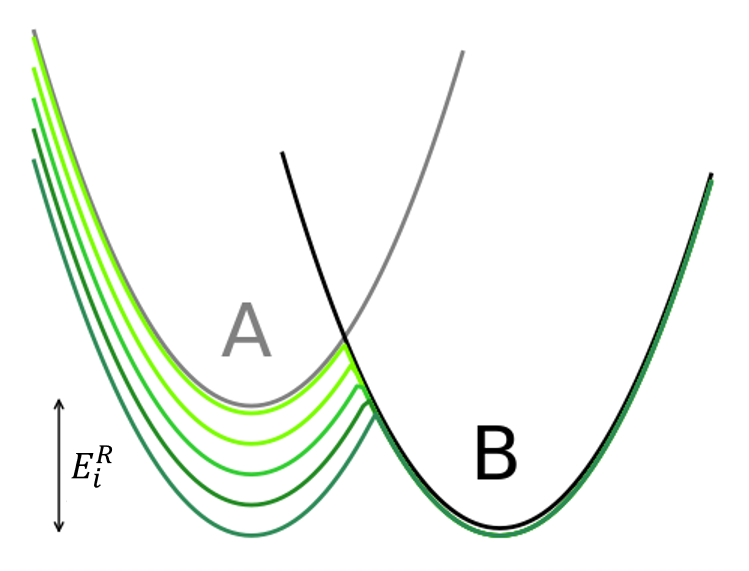
\includegraphics[width=\textwidth]{fig/intro/EDS_parmeters_Eoff.png}
        \caption{Effect of $E_i^R$ on $V_R$}
        \label{fig: EDS_potential_behaviourb}
    \end{subfigure}
    \end{center}
    \caption{Schematic illustration of the effect of the two types of EDS reference-state parameters. (a) The smoothing parameter $s$ decreases the barriers between the end states. If $s$ is too small, an ``undersampling'' situation occurs with a global unphysical minimum. (b) The energy offsets $\vec{E}^R$ provide equal weighting to all end states in the EDS reference state.  The figure was generated with Ensembler \cite{Ries2021A}.}
    \label{fig: EDS_potential_behaviour}
\end{figure}

% laws of motion of R
The force on a particle $k$ in the EDS reference state is calculated as \cite{Christ2008},
\begin{equation}
    \vec{f}_k(t)=-\frac{\partial V_R(\vec{r}; s, \vec{E}^R)}{\partial \vec{r}_k} = \sum^N_{i=1}\frac{e^{-\beta s(V_i(\vec{r}) -E_i^R)}}{\sum^N_{j=1}{e^{-\beta s (V_j(\vec{r})-E_j^R)}}}  \left( -\frac{\partial V_i(\vec{r})}{\partial \vec{r}_k} \right) \,.
    \label{eq:laws_of_motion}
\end{equation}
%
For $s$ values close to one, the reference-state forces are dominated by the one end state, for which the current coordinates are most favourable, while the other end states give high energies and therefore contribute little (i.e. ``dummy states'').  
For small $s$ values (undersampling situation), all end states contribute effectively to the forces, resulting in the global unphysical minimum.

%% ddFE
The free-energy difference between two end states $A$ and $B$ can be calculated by employing the Zwanzig equation twice forming a path via the reference state~$R$ \cite{Zwanzig1954,Christ2007,Christ2008},

%published & constantly cited form by Clara christ:
%% - \frac{1}{\beta} \ln(\frac{⁡\langle e^{-\beta (V_B-V_R)}\rangle_R}{\langle e^{-\beta (V_A-V_R )}\rangle_R})
\begin{align} \nonumber
    \Delta G_{\text{BA}} &=  \Delta G_{\text{BR}} + \Delta G_{\text{RA}} \\ 
    &=-\frac{1}{\beta}\left(\ln \langle e^{-\beta (V_B-V_R)}\rangle_R - \ln \langle e^{-\beta (V_A-V_R )}\rangle_R\right) \\ 
    &= -\frac{1}{\beta} \ln \frac{\langle e^{-\beta (V_B-V_R)}\rangle_R}{\langle e^{-\beta (V_A-V_R)}\rangle_R}.
    \label{EQ: Free Energy calculation via reference state}
 \end{align}

%---------------------------
\FloatBarrier

\subsection{Replica-Exchange EDS (RE-EDS)}
The recently introduced RE-EDS method \cite{Sidler2016,Sidler2017} is a type of Hamiltonian replica exchange \cite{Hansmann1997,Sugita2000} with the smoothness parameter $s$ as the exchange dimension ($1 \geq s > 0$), which was inspired from constant pH simulations by Lee \textit{et al.} \cite{Lee2014,Lee2015}. The approach is shown schematically in Figure \ref{fig:RE-EDS_Scheme}.
RE-EDS does not require a single (optimal) $s$-value. Instead enhanced sampling is achieved by exchanging between the replicas with different smoothness levels. This simplifies the parameter choice problem and thus, the method can be applied to systems with more than two end states \cite{Sidler2016,Sidler2017}.

%Exchange criterium
For the pairwise exchanges between neighboring replicas $k$ and $l$, a Metropolis-Hastings criterion \cite{Hastings1970} is used \cite{Sidler2016,Sugita2000},
\begin{equation}
    \begin{split}
    p_{k,l} = min\bigg(1, \exp \Big[
                &-\beta ((H_{R}(\vec{r}_k; s_l)+H_{R}(\vec{r}_l; s_k))\\
                &-(H_{R}(\vec{r}_l; s_l)+H_{R}(\vec{r}_k; s_k))  \Big] \bigg) ,
    \end{split}
\end{equation}
where $H_{R_k}$ and $H_{R_l}$ are the reference-state Hamiltonians of the respective replicas, $\vec{r}_k$ and $\vec{r}_l$ are the current coordinates of the replicas.

Replicas are placed between $s=1.0$ and a lower bound of $s$, where the reference state is in undersampling. The replicas with low $s$ values facilitate the transitions between the low-energy regions of the  different end states. Especially for systems with slowly adapting environments (e.g. protein binding pockets), regions in $s$-space with very low acceptance probability can occur. Thus, to ensure sufficient exchanges between all pairs of replicas, a local variant of the round-trip time optimization algorithm \cite{Katzgraber2006, Nadler2008} was developed to optimally place the replicas in $s$-space \cite{Sidler2017}.
It was found that a single set of energy offsets can be used for all replicas \cite{Sidler2016}. However, it is important that these energy offsets are chosen well to avoid ``leakage'' effects, resulting in one or more end states not being properly sampled \cite{Sidler2016}.
The final free-energy differences are estimated from the replica at $s=1.0$, which represents the physical minima of the end states.

\begin{figure}[h]
    \centering
    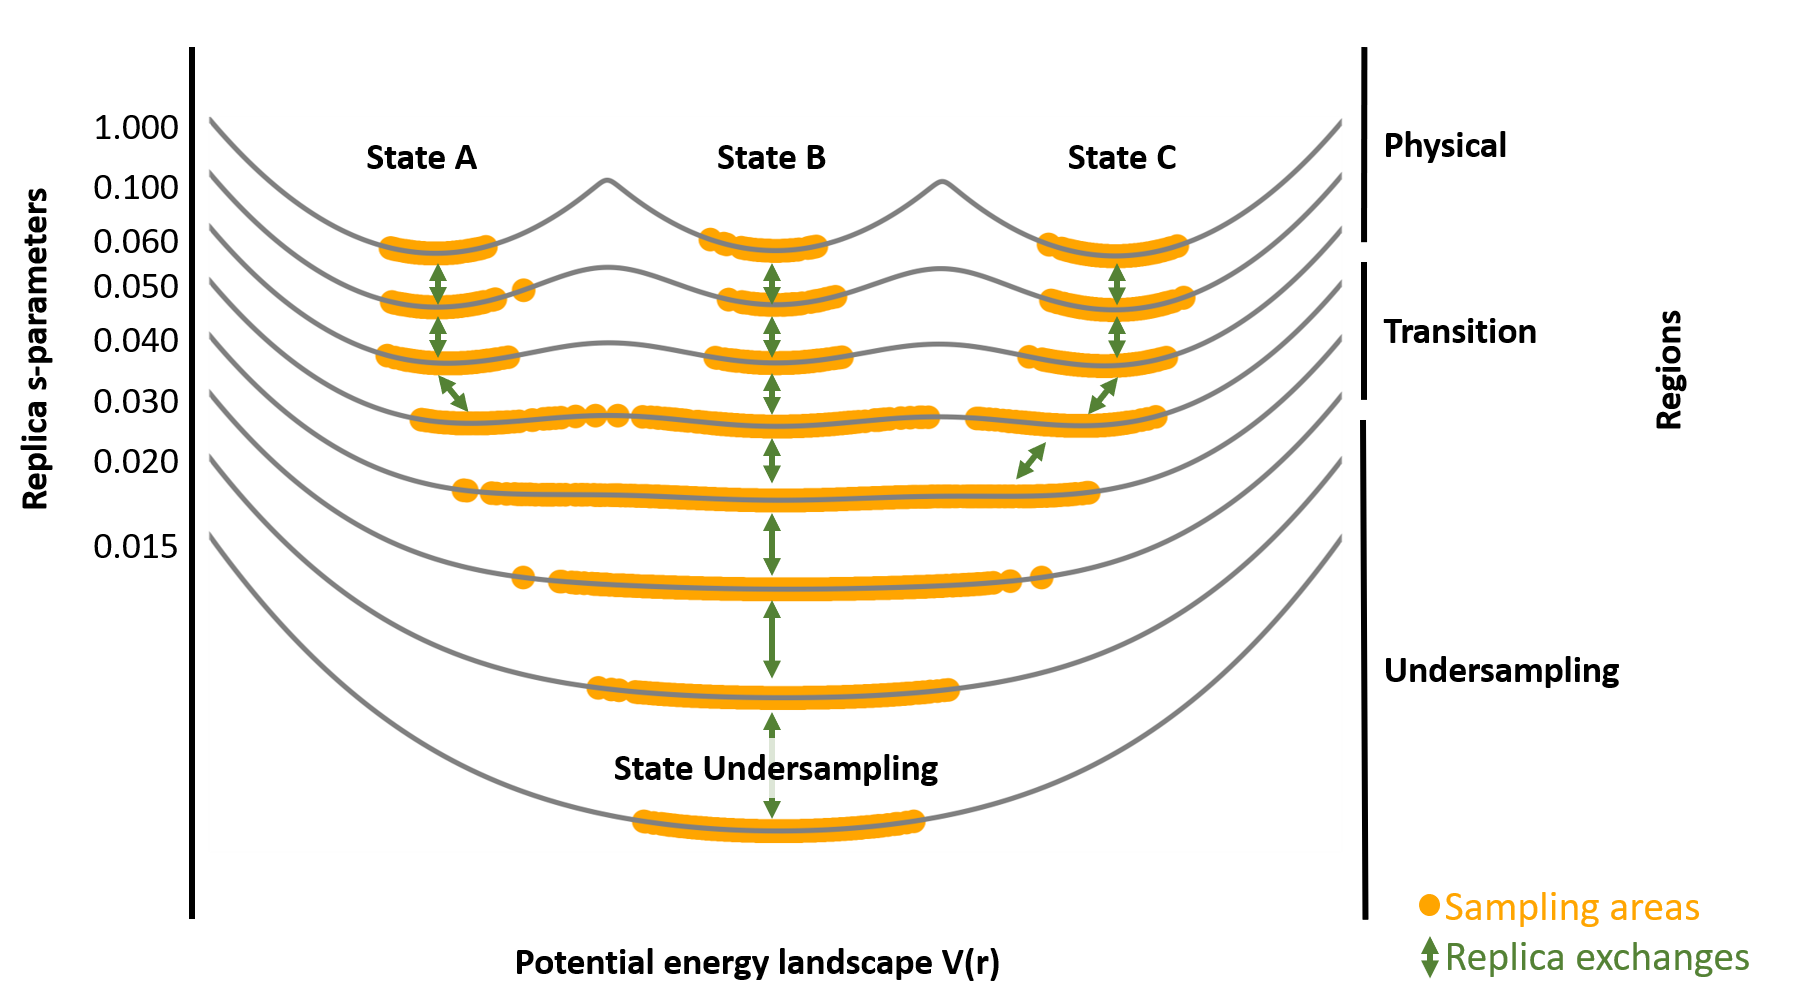
\includegraphics[width=\columnwidth]{fig/theory/Reeds_scheme_first.png}
    \caption{Schematic illustration of RE-EDS with three harmonic oscillators as end states ($A$, $B$, and $C$). Each replica differs by the $s$-parameter, generating reference states with a different degree of smoothness. Sampling of each replica is denoted with orange dots. Exchanges between the replicas are indicated with green arrows. The replica graph shows three regions: a ``physical'' region where $s$ is close to 1, a transition region, and the ``undersampling'' region when $s$ approaches zero. The figure was generated with Ensembler \cite{Ries2021A}.}
    \label{fig:RE-EDS_Scheme}
\end{figure}

%---------------------------
\FloatBarrier

\subsection{Automatic Parameter Optimization}
To facilitate the determination of the energy offsets and $s$-parameter distribution, we have extended and further automatized the previous \cite{Sidler2017} RE-EDS workflow (Figure \ref{fig:Workflow}).
\begin{figure}[h!]
    \centering
    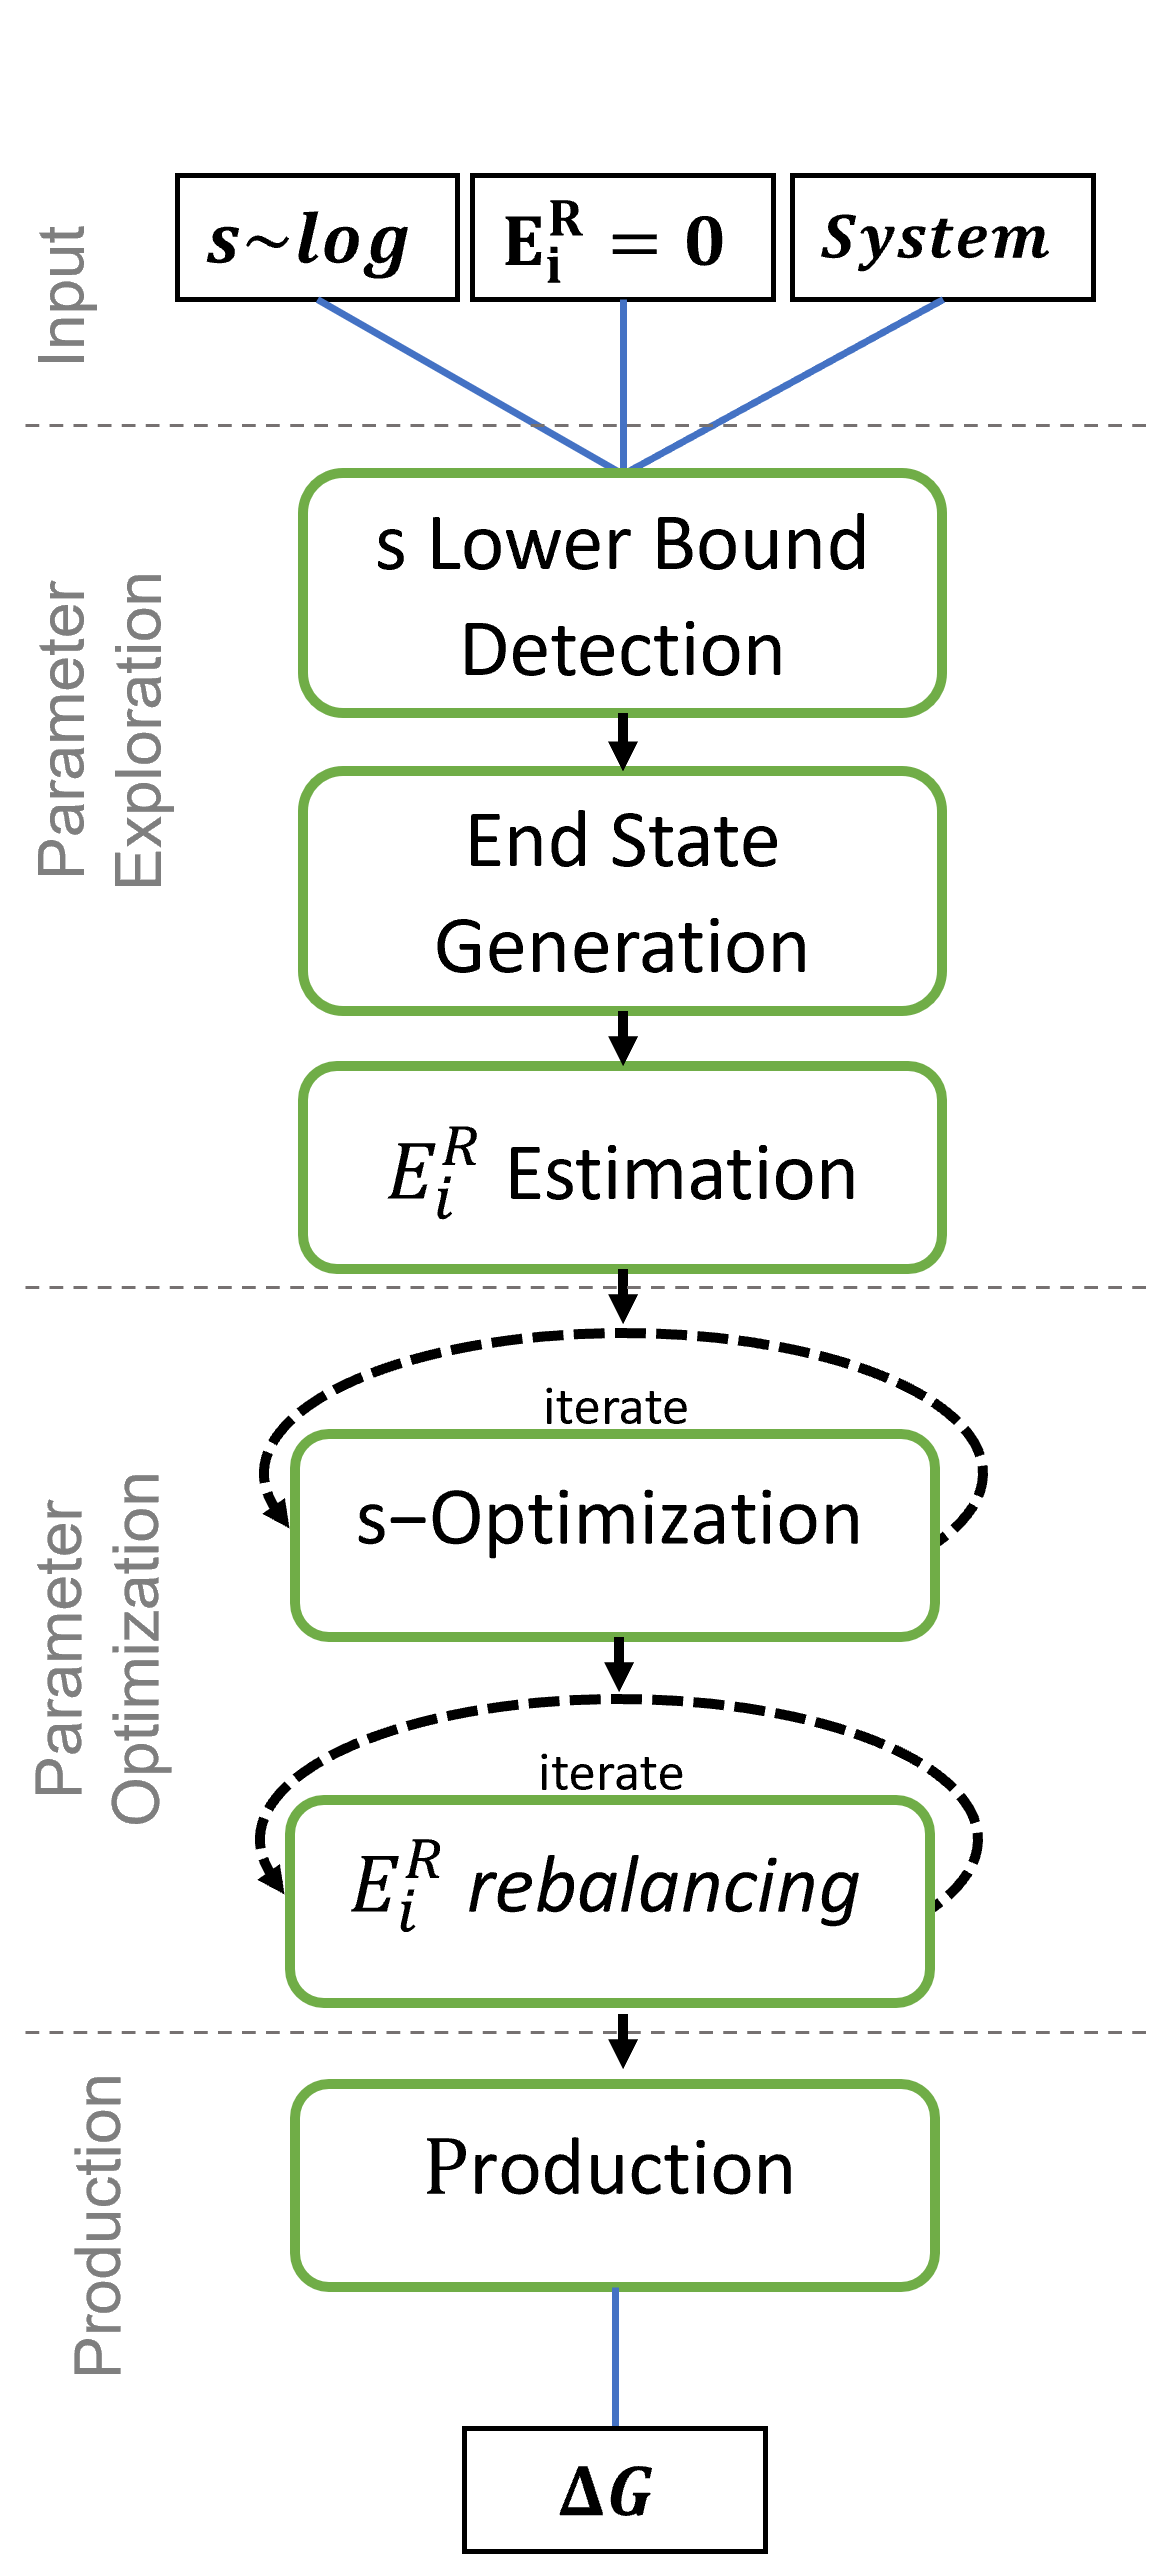
\includegraphics[width=0.5\columnwidth]{fig/theory/RE_EDS_Pipeline.png}
    \caption{The RE-EDS workflow can be split into four steps: (1) Input stage with energy offsets set to $E_i^R=0$ and a set of $s$-parameters logarithmically distributed between $1$ and $10^{-5}$; (2) Parameter exploration to determine the lower bound for $s$, to obtain equilibrated coordinates for each end state, and to estimate initial energy offsets with the PEOE scheme \cite{Sidler2016}; (3) Parameter optimization to improve the $s$-distribution with the N-LRTO algorithm \cite{Sidler2017} and the state sampling with energy offset rebalancing; (4) Production run and calculation of the free-energy differences.}
    \label{fig:Workflow}
\end{figure}

%
The initial input for a system with $N$ end states consists of a prepared EDS system (i.e. topology,  perturbation topology, initial coordinates, and distance restraints), a list of energy offsets of length $N$ with $E_i^R = 0; ~ \forall ~ i \in [1,...,N]$, and a list of $s$-parameters, which are logarithmically distributed in the range $s_i \in [1, 10^{-5}]$. Typically, we use 21 initial $s$ values. 

The parameter exploration consists of three substeps: (i) determining the lower bound for the $s$-distribution (newly introduced), (ii) obtaining optimized coordinates within the EDS set-up for each end state (newly introduced), and (iii) estimation of an initial set of energy offsets (as done previously in Ref.~\cite{Sidler2016}).

%%1. initial parameter search
To enable sampling of all end states at $s=1.0$, some replicas have to be in undersampling to facilitate transitions. However, for efficiency reasons (and numerical stability) the number of replicas $M$ in undersampling should be small and the lowest $s$-value should be as high as possible. From a short simulation with the initial $s$-distribution between $[1, 10^{-5}]$, the highest smoothing parameter $s_{M_\mathrm{us}}$ at which undersampling still occurs is determined and used in the following as a lower bound for the $s$-distribution. The $s$-distribution for the next step is then defined by logarithmically distributed replicas between $s=1.0$ and the automatically determined lower bound.

%%%state optimization
Optimized coordinates for each end state in the EDS setup can be automatically obtained by short parallel simulations, where one end state in turn is favoured by setting an arbitrarily large energy offset for this state. 
The optimized coordinates allow the user to start RE-EDS simulations from different end states and are needed for the subsequent parameter optimization. 

 %%% estimate EOFFs:
In the last substep, $E_{\text{i}}^{\text{R}}$ estimation, the previously developed parallel energy offset estimation (PEOE) \cite{Sidler2016} scheme is used to estimate the initial set of energy offsets. This is done based on a short simulation with the initial parameters. For each replica $k$ in the undersampling region, the energy offsets are extracted using \cite{Sidler2016},
\begin{equation}
    E_{i}^{R}(new)=-\frac{1}{\beta}\ln \Big < e^{-\beta \big(V_i(\vec{r})-V_R(\vec{r}; s_{k},\vec{E}^{R}(old))\big)}\Big>_{R(s_{k},\vec{E}^{R}(old))} .
    \label{eq: EoffEstimator}
\end{equation}
The energy offsets that were extracted in parallel for the $k$ replicas are subsequently averaged and used as initial set of energy offsets. These energy offsets should provide a first solution that is close to the optimal choice of energy offsets, which leads to an optimal state sampling of all end states in the RE-EDS simulation. As the initial energy offsets are obtained from the replicas in undersampling, they may not be exactly optimal and require fine-tuning in the next phase. 


%%2. optimization of parameters
In the second step of the RE-EDS workflow, first the $s$-distribution is optimized and subsequently the energy offsets are fine tuned.
%
%%% s-Optimization:
The $s$-distribution is improved by minimizing the round-trip time $\tau$ and increasing the number of round-trips, using the multistate local round-trip time optimization (N-LRTO) algorithm \cite{Sidler2017}. The optimization is performed in an iterative manner with short simulations.
This step is required as exchange bottlenecks between two replicas might occur leading to a very slow round trip time or to no round trips at all. 
In the N-LRTO algorithm, new replicas are inserted in each iteration by linear interpolation in the $s$-regions with exchange bottlenecks, while the replica positions of the previous iteration are retained. Adding replicas theoretically increases the round-trip time because of a longer path between the top and bottom replicas. However, the addition of intermediate replicas also increases the exchange probability between neighboring replicas, thus reducing the round-trip time. With the optimization algorithm, we aim to determine the balance between the length of the replica path and the likelihood of exchange between replicas for minimal round-trip time. The exchange bottlenecks are identified for each end state separately (i.e. multistate). The number of replicas added can be chosen by the user. The iteration is stopped when the average round-trip time $\overline{\tau}$ converges. 
The N-LRTO variant is needed for systems for which severe bottlenecks are observed with the initial logarithmic $s$-distribution (e.g. protein binding pockets). For systems with smaller perturbations, the global multistate variant (N-GRTO) \cite{Sidler2017} can be more efficient as this algorithm re-distributes the replicas in $s$-space according to the exchange statistics. %In very severe cases, this can lead to an oscillating behavior, as one bottleneck is fixed, but another appears due to an imbalance of replica shifting.
%
In this study, we started with the same number of replicas as used for the PEOE scheme above and added four replica positions per iteration in the N-LRTO algorithm.

%%%% Eoff Rebalancing:
After optimizing the number of round trips and $\tau$, the distribution of the state sampling is improved. To reach the ideal situation that each end state is sampled to an equal amount, the initial energy offsets need to be fine tuned, while keeping the round trips approximately constant. For this, we introduce here the energy offset rebalancing scheme.
To avoid overshooting, a correction factor is calculated and applied iteratively,
\begin{equation}
    \Delta E^{corr}_i = - \frac{1}{\beta} \ln \left( \frac{f_i^{\text{mc}}+c}{f^{\text{mc,ideal}}_{i}+c} \right),
    \label{eq: EoffRebalancing}
\end{equation}
where $f_i^{\text{mc}}$ is the current sampling fraction (or estimated probability) of an end state contributing to $V_R $, and $f^{\text{mc,ideal}}$ is the ideal sampling fraction (see Section \ref{metrics}). 
%
To make the approach more robust, a pseudo count $c$ is introduced to avoid singularities with zero sampling, which is defined as,
\begin{equation}
    c = \frac{f^{\text{mc,ideal}}}{x},
    \label{eq: EoffRebalancingPseudoCount}
\end{equation}
with the intensity factor $x$.
The default of the pseudo count was chosen to result in a maximal correction of $\Delta E^{corr}_i=8.43$~kJ/mol, corresponding to a minimum 30-fold reduced sampling compared to the expected optimal sampling.

%%% 3. production run
After optimizing the RE-EDS parameters, the production run is performed for a chosen length. 
The free-energy differences are subsequently calculated using the replica at $s=1.0$ with Eq.~(\ref{EQ: Free Energy calculation via reference state}).

\subsubsection{Starting State Mixing}
The sampling in RE-EDS simulations can be further improved by using starting coordinates for the replicas corresponding to the different end states (i.e. replica 1 starts in a low-energy configuration for end state 1, replica 2 in a low-energy configuration for end state 2, etc.). This technical approach is called ``starting state mixing'' (SSM) in the following and is also used for Hamiltonian replica-exchange TI calculations (see e.g. \cite{Graf2016, Hahn2020}). The optimized coordinates obtained in the parameter exploration step can be used for SSM. We compare RE-EDS simulations with SSM and with a single set of starting coordinates (abbreviated as 1SS).  

\subsubsection{Analysis}
\label{metrics}
Three types of metrics were used to quantify the sampling in RE-EDS simulations. The first metric determines for each end state $i$ the sampling fraction where it is maximally contributing to the reference state, i.e. $f_i^{\text{mc}}$. A maximally contributing state is defined as the end state with the lowest potential energy minus its energy offset in a frame. As can be seen in  Eq.~\eqref{eq:laws_of_motion}, maximally contributing end states have the largest impact on the reference-state sampling at a given time point.

%
Optimal sampling in a RE-EDS system is achieved when all end states are sampled as maximally contributing states to an equal extent at $s=1.0$, i.e. 
\begin{equation}
f_{i}^{\text{mc,ideal}} = \frac{1}{N} ~, \forall ~ i~\in~ \{1, ..., N\}
\label{eq: optimalDominationSamplingDist}
\end{equation}

The second metric is the estimated sampling fraction of ``physical occurrence'' of an end state $i$, i.e. $f_i^{\text{occur}}$. As a result of phase-space overlap with the current maximal contributing end state, other end states in the EDS system might be sampled simultaneously. An end state is counted as ``occurred'' when its potential energy is below the threshold $V_i \leq T_{i}^{\text{phys}}$ at a time point $t$. 
These thresholds are estimated during the second substep of the parameter exploration phase. If end states show no phase-space overlap, $f_i^{\text{occur}}$ will be (nearly) the same as $f_i^{\text{mc}}$. 

Undersampling is detected with a third metric using the thresholds $T_{i}^{\text{us}}$. These thresholds are determined in the first substep of the parameter exploration phase from the simulation with the lowest $s$-value. If all end states have a potential energy below their respective $V_i - E^R_i \leq T_{i}^{\text{us}}$, the current frame is characterized as undersampling. \cite{Sidler2016} 

\FloatBarrier